\documentclass[10pt,a4paper,ssfamily]{exam}
\usepackage[numbers,sort&compress]{natbib}
\usepackage[utf8]{inputenc}
\usepackage[brazil]{babel}
\renewcommand{\baselinestretch}{1.15}
\usepackage{epsfig}
\usepackage{nicefrac}
\usepackage{graphicx}
\usepackage{makeidx}
\usepackage{multicol}    
\usepackage{multirow}
\usepackage{amssymb}
\usepackage{enumitem}
\usepackage{xcolor}
\usepackage{lmodern}
\usepackage{scrextend}
\usepackage{xcolor}
\usepackage[hidelinks]{hyperref}
\usepackage{amsmath}
\usepackage{mathtools}
\usepackage{chemformula}
\usepackage{mhchem}
\renewcommand{\t}{\text}
\newcommand{\listfont}{\bf\fontencoding{OT1}\sffamily\large}
\newcommand{\titlesfont}{\fontencoding{OT1}\sffamily\large}
\renewcommand{\baselinestretch}{1.24}
\newcommand{\oC}{$^\circ$C}
\newcommand{\sen}{\textrm{sen }}
\newcommand{\Mg}{Mg$^{2+}$}
\newcommand{\sol}[1]{\href{http://m3g.github.io/didatico/qf935/atividades/#1.f90}{Solução}}
\newcommand*{\LargeCdot}{\raisebox{-0.25ex}{\scalebox{1.2}{$\cdot$}}}

% Activity envinronment

\newsavebox{\fmbox}
\newenvironment{ex}
{\begin{center}\vspace{0.3cm}\begin{lrbox}{\fmbox}\begin{minipage}{12cm}{\bf Atividades}
\begin{enumerate}\setcounter{enumi}{\exnumber}}
{\global\chardef\exnumber=\value{enumi}\end{enumerate}\end{minipage}\end{lrbox}\fbox{\usebox{\fmbox}}\vspace{0.3cm}\end{center}}

% Code blocks definitions

\usepackage{listings}

\renewcommand{\t}{\textrm}
\lstnewenvironment{code}{\lstset{language=[90]Fortran,
  basicstyle=\ttfamily,
  keywordstyle=\color{blue},
  commentstyle=\color{gray},
  identifierstyle=\color[RGB]{0,102,0}\textbf,
  xleftmargin=1.5cm,
  showstringspaces=false,
  morecomment=[l]{!\ }% Comment only with space after !
}}{}

\lstdefinestyle{code}{
  language=[90]Fortran, 
  basicstyle=\ttfamily,
  keywordstyle=\color{blue},
  commentstyle=\color{gray},
  identifierstyle=\color[RGB]{0,102,0}\textbf,
  xleftmargin=1.5cm,
  showstringspaces=false,
  morecomment=[l]{!\ }% Comment only with space after !
}
\newcommand{\codefile}[1]{\lstinputlisting[style=code]{#1}
            \begin{center}
            \href{http://m3g.github.io/didatico/simulacoes/#1}
                 {\textcolor{blue}{[Clique para baixar o código]}}
            \end{center}}

\newcommand{\codelink}[1]{
            \begin{center}
            \href{http://m3g.github.io/didatico/simulacoes/#1}
                 {\textcolor{blue}{[Clique para baixar o código]}}
            \end{center}}

\begin{document}

\pagestyle{plain}

% Start exercise counter
\global\chardef\exnumber=0

\sffamily
\pagestyle{empty}

\begin{enumerate}
\item
Um canhão lança uma bala do chão, como mostra a figura abaixo.
\begin{center}
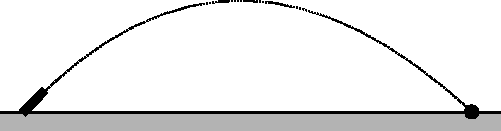
\includegraphics[width=8cm]{./figuras/canhao.pdf}
\end{center}
A força da gravidade acelera a bala para baixo, de acordo com a
aceleração da gravidade, que é $g = 9.8$~m/s$^2$. A velocidade da bala é
dada por um vetor, porque ela tem duas direções, $x$, e $y$. A bala é
atirada da posição $(0,0)$, e com velocidade inicial $(10,10)$. O
movimento é acelerado apenas na direção $y$, e para baixo. Na direção
$x$ o movimento tem, portanto, velocidade constante, e o movimento é
descrito pela fórmula $s = s_0 + v_0 t$. Na direção $y$ o movimento é
acelerado pela gravidade, portanto a fórmula que descreve o movimento é
$s = s_0 + v_0t + (a/2)t^2$.
\begin{enumerate}
\item
Faça um programa que faça as contas para calcular a posição $(x,y)$ da
bala em qualquer valor de tempo, $t$, que você definir.
\item
Sofistique o seu programa para calcular a trajetória da bala, isto é,
que salve três vetores, um de tempo, e outros de posições $x$ e $y$.
\item
Encontre em que tempo a bala chega ao chão. 
\item
Como variam o tempo e a distância horizontal (em $x$) 
em que bala chega ao chão se você varia o ângulo de lançamento
(para uma velocidade com mesmo módulo)?
\end{enumerate}

\item
A força gravitacional aponta para o centro da terra. Ela tem a forma
\[
F = G \frac{m_1 m_2}{r^2}
\] 
onde $G$ é uma constante, $m_1$ e $m_2$ são as massas dos dois corpos (a
terra é o outro objeto), e $r$ a distância entre eles. A constante $G$
vale $G = 6.67\times 10^{-11}$m$^3/$kg~s$^2$. A massa da terra é
$5.97\times 10^{24}$kg, e o raio da terra é $6371$~km, ou 
$6.371 \times 10^{6}$m.
Vamos imaginar que o centro da terra está na posição $x=(0,0)$, e que o
temos um objeto que pesa 1 kg, e trabalhar com uma representação da
terra em duas dimensões. 
\begin{enumerate}
\item
Faça um código que calcule a força que age sobre o corpo, na situação
da figura (a) ilustrada abaixo. Note que a coordenada $x$ do objeto é
zero, e que $y$ é a soma da altura do objeto com o raio da terra. 
\begin{center}
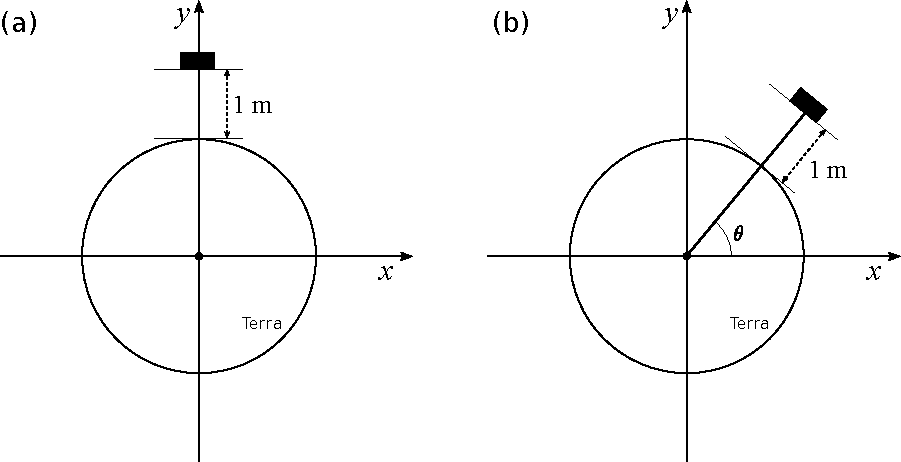
\includegraphics[width=12cm]{./figuras/terra.pdf}
\end{center}
\item
Modifique o seu programa para tentar calcular a força que atua sobre o
corpo quando ele está em qualquer lugar da terra, mas a uma altura de
1~m, como ilustrado na figura (b). As posições $x$ e $y$ agora dependem
do ângulo $\theta$, como ilustrado na figura. 
\end{enumerate}

\item
A força que você calculou no exercício anterior aponta sempre para o
centro da terra. Como mostra a figura abaixo, ela pode ser decomposta em
duas componentes, $F_x$ e $F_y$, que dependem do mesmo ângulo $\theta$
da figura.
\begin{center}
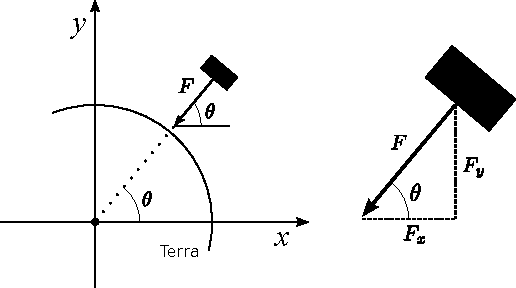
\includegraphics[width=12cm]{./figuras/terra2.pdf}
\end{center}
\begin{enumerate}
\item
Faça o seu programa calcular cada uma das componentes separadamente.
\item
Calcule a aceleração em cada direção, separadamente, no mesmo programa.
\item
O movimento é acelerado nas duas direções, $x$ e $y$. Portanto, a queda
do corpo obedece a lei $s = s_0 + v_0 + at^2/2$ para cada direção.
Adicione ao seu programa a conta que calcula a posição (tanto em $x$
como em $y$) do corpo para qualquer instante de tempo. Assuma que a
velocidade inicial do corpo é nula (ou seja, ele começa parado). Preste
atenção que as posições vão ser em relação ao centro da terra.  
\end{enumerate}

\item
Na figura abaixo representamos a Terra e a Lua. Para facilitar as
contas, vamos representar todos os números com unidades mais
convenientes. Vamos contar a massa da Terra e da Lua usando como unidade
a massa da terra. Desta forma, $m_{\textrm{Terra}} = 1$ e a massa da
Lua, que é $m_{\textrm{Lua}} = 7.36\times 10^{22}$~kg, vai ser 
$m_{\textrm{Lua}} = 0.0123$ (veja a massa da Terra no exercício 2.
A distância entre a Terra e a Lua é de 384400~km. Vamos medir essa
distância em ``raios da Terra''. O raio da Terra é 6371~km, portanto a
distância entre a Terra e a Lua é $\sim$60 vezes o raio da Terra (a Lua
está bem longe, né?). 
\begin{center}
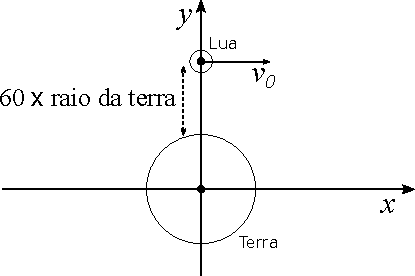
\includegraphics[width=6cm]{./figuras/terra_e_lua.pdf}
\end{center}
A Lua gira em torno da Terra com uma velocidade de aproximadamente 3600~km/h. 
Também vamos escrever essa velocidade usando o raio da Terra
como medida de distância. Portanto, a velocidade é 0.565 ``raios da
Terra'' por hora. Nestas mesmas unidades, a constante da gravitação,
$G$, vale $G = 19,968~r_{\textrm{Terra}}^3~ m_{\textrm{Terra}}^{-1}$~h$^{-2}$.

O objetivo é fazer um gráfico da posição $(x,y)$ da Lua em torno da
Terra, no decorrer de um dia.

\item
Agora, sofistique o seu programa para que a Terra não esteja fixa no
centro, mas se mova também em função da atração que a Lua exerce sobre
ela.



\end{enumerate}




\end{document}


